%%%%%%%%%%%%%%%%%%%%%%%%%%%%%%%%%%%%%%%%%%%%%%%%%%%%%%%%%%%%%%%%%%%%%%%%%%%%
%%%%%                          ANNEXE 5                               %%%%%%
%%%%%%%%%%%%%%%%%%%%%%%%%%%%%%%%%%%%%%%%%%%%%%%%%%%%%%%%%%%%%%%%%%%%%%%%%%%%

\appendix
\renewcommand\chaptername{Annexe~}
\phantomsection 

\lhead[\fancyplain{}{\leftmark}]%Pour les pages paires \bfseries
      {\fancyplain{}{}} %Pour les pages impaires
\chead[\fancyplain{}{}]%
      {\fancyplain{}{}}
\rhead[\fancyplain{}{}]%Pour les pages paires 
      {\fancyplain{}{\rightmark}}%Pour les pages impaires \bfseries
\lfoot[\fancyplain{}{}]%
      {\fancyplain{}{}}
\cfoot[\fancyplain{}{\thepage}]%\bfseries
      {\fancyplain{}{\thepage}} %\bfseries
\rfoot[\fancyplain{}{}]%
     {\fancyplain{}{\scriptsize}}


%%%%%%%%%%%%%%%%%%%%%%%%%%%%%%%%%%%%%%%%%%%%%%%%%%%%%%%%%%%%%%%%%%%%%%%%%%
%%%%%                      Start part here                          %%%%%%
%%%%%%%%%%%%%%%%%%%%%%%%%%%%%%%%%%%%%%%%%%%%%%%%%%%%%%%%%%%%%%%%%%%%%%%%%%

\chapter{Dimensionnement analytique des lames de l'OB}
\label{Ann:5_Dimensionnement analytique des lames de l'OB}

\minitoc
\newpage

%/!\/!\/!\/!\/!\/!\/!\/!\/!\/!\/!\/!\/!\/!\/!\/!\/!\/!\/!\/!\/!\/!
	\section{Dimensionnement des lames flambées}
	\label{sec:4.3:Dimensionnement des lames flambées}
%/!\/!\/!\/!\/!\/!\/!\/!\/!\/!\/!\/!\/!\/!\/!\/!\/!\/!\/!\/!\/!\/
    %/////////////////////////////////////////////
	\subsection{Modèle analytique statique approché} 
    %/////////////////////////////////////////////
       	%*************
		\subsubsection{Établissement du modèle statique} 
		%*************		
	Nous avons précédemment simulé l'évolution du comportement statique d'une telle structure, en imposant des incréments de niveau de flambement. Il serait intéressant maintenant d'être capable de trouver la bonne géométrie pour les lames, en connaissant simplement le niveau énergétique injecté dans le bistable par l'oreille. Ce niveau résulte directement des paramètres $K$,$L$ et $x_0$ qui ont été définis précédemment. On aimerait alors lier ces trois paramètres à $K_{\varphi}$ et aux paramètres géométriques, ainsi que les paramètres matériau de d'une lame. Cette étape simplifierait le temps de dimensionnement des lames pour des niveaux d'entrée énergétiques différents.\\
%%%%%%%%%%%
\begin{figure}[!htbp]
\begin{center}
    \captionsetup{justification=centering}
	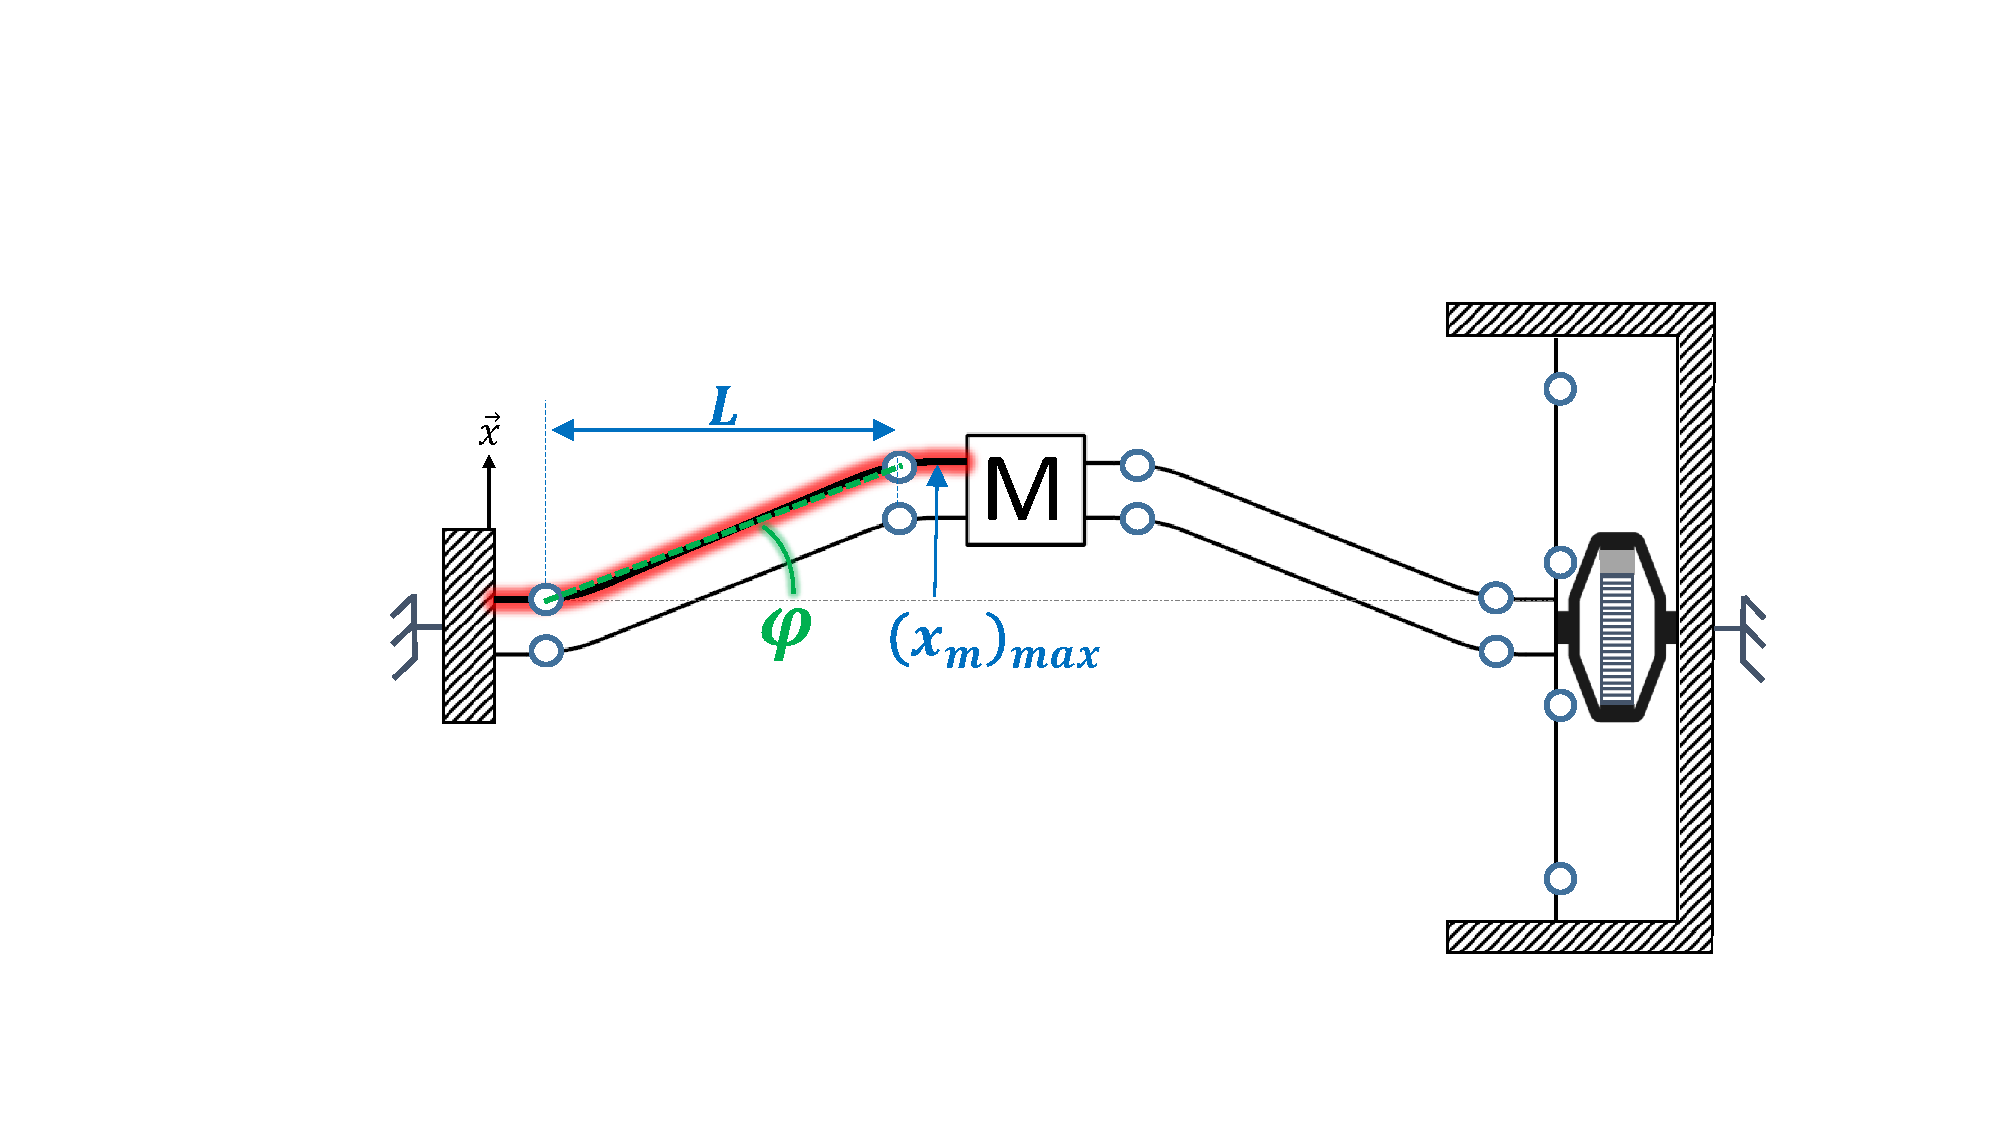
\includegraphics[trim={6cm 2.8cm 4cm 5cm},clip, width=0.7\textwidth]{../Chap4/Figure/OB_surbrillance_1_lame.pdf}
	\caption{L'OB à l'équilibre en $x_0$}
	\label{fig:OB_surbrillance_1_lame}
\end{center}
\end{figure}
%%%%%%%%%%%
Dans un souci de symétrie, le comportement mécanique de chacune des 4 lames est identique. Nous allons donc isoler le comportement d'une seule lame, mise en surbrillance sur la figure \ref{fig:OB_surbrillance_1_lame} pour établir un modèle analytique.
L'épaississement local aura pour rôle de rigidifier les pivots souples car la lame sera plus difficilement déformable sur cette portion. Cela dit il est important d'épaissir la lame localement, afin de minimiser l'impact des déformation résiduelles dues à la fabrication. L'idéal serait d'épaissir la lame de façon à minimiser l'impact sur la rigidité de la lame en flexion. C'est en effet possible si on arrive à épaissir la portion de la lame qui ne subit pas de déformation sous la sollicitation qui lui est demandée.
%%%%%%%%%%%%%%%%%%%%%
\begin{figure}[!htbp]
\begin{center}
    \captionsetup{justification=centering}
	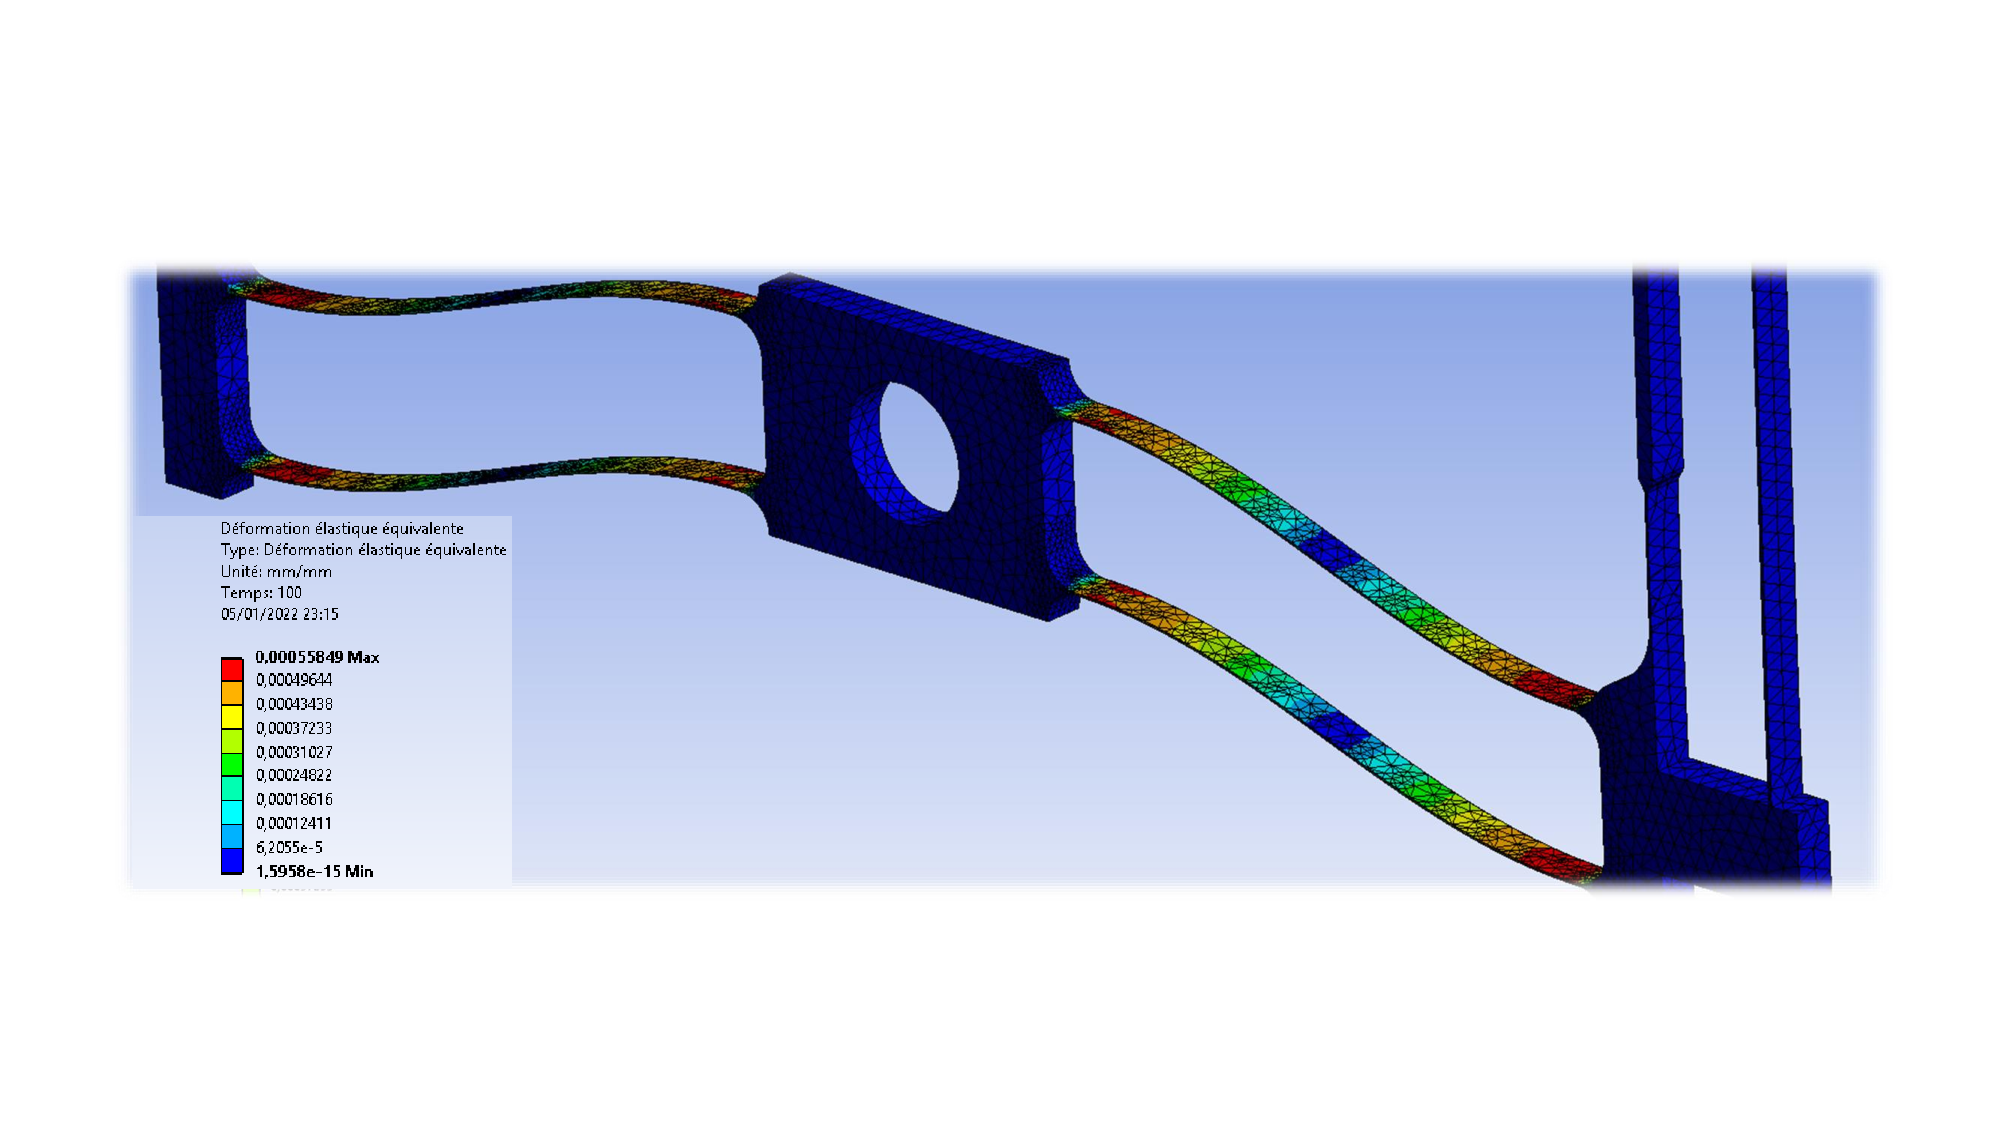
\includegraphics[trim={2cm 4cm 2cm 4cm},clip, width=\textwidth]{../Chap4/Figure/ANSYS_deformation.pdf}
	\caption{Déformation des lames horizontales sans épaississement}
	\label{fig:ANSYS_deformation}
\end{center}
\end{figure}
%%%%%%%%%%%
Sur la figure \ref{fig:ANSYS_deformation} on peut voir la déformation structurelle des lames horizontales sans épaississement, pour les mêmes conditions initiales et sollicitations externes que le modèle avec épaississements. On s'aperçoit alors que les déformations sont principalement concentrées aux extrémités des lames et sur un large portion au centre la lame subit des déformations 5 à 10 fois plus faibles. Le modèle analytique sera donc sous-dimensionné par rapport au modèle avec épaississements. Il suffira alors d'appliquer un coefficient de correction qui pourra être vérifié avec la méthode numérique développée précédemment.\\
	Sachant que le comportement des lames est linéaire sur toute la plage de fonctionnement, nous allons nous placer dans le cas extrême de $x_m = (x_m)_{max}$ et isoler une seule lame. Dans cette configuration, la lame peut être décomposée en deux lames symétriques encastrées-libres tel qu'on voit que la figure \ref{fig:OB_surbrillance_2_lames}. Leur longueur vaut alors $L/2$ et leur flèche à l'extrémité libre atteint pour chacune des lames :
\begin{equation}
		x_E =\frac{(x_E)_{max}}{2}
\label{eq:x_E=x_max/2}
\end{equation}
On introduit aussi la force normale $F_E$ qui induit cette flèche à l'équilibre statique, et depuis laquelle découlera la rigidité en flexion d'une demi-lame.\\
%%%%%%%%%%%
\begin{figure}[!htbp]
\begin{center}
    \captionsetup{justification=centering}
	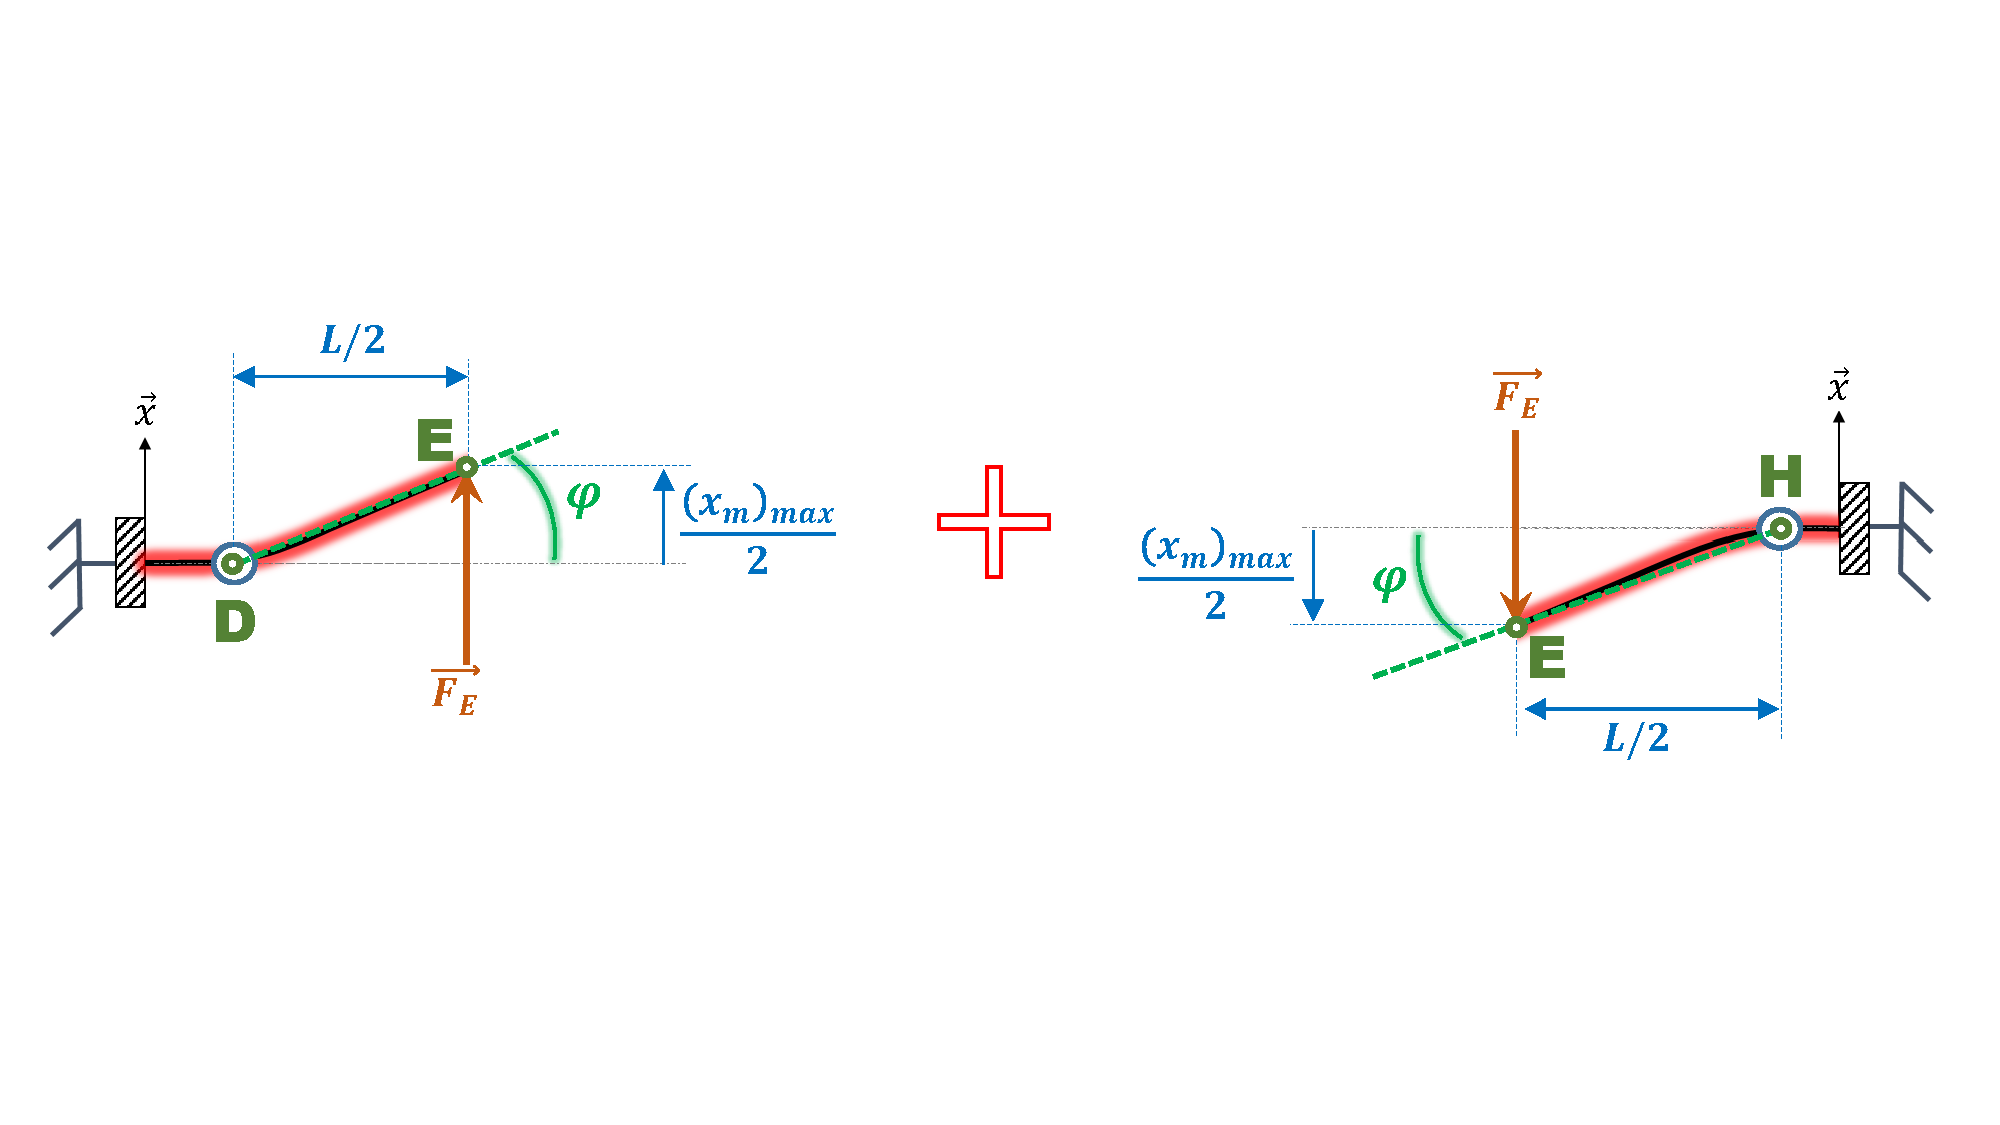
\includegraphics[trim={0cm 6cm 1cm 5cm},clip, width=\textwidth]{../Chap4/Figure/OB_surbrillance_2_lames.pdf}
	\caption{Hypothèse du comportement statique d'une lame de l'OB}
	\label{fig:OB_surbrillance_2_lames}
\end{center}
\end{figure}
%%%%%%%%%%%
Sur figure \ref{fig:poutre_flexion_simple} on montre le schéma de modélisation pour la demi-lame gauche. Naturellement le résultat sera similaire pour la demi lame droite par symétrie. On se positionne dans la théorie de déformation des poutres d'Euler-Bernoulli sans gauchissement pour la suite de l'étude analytique. 
%%%%%%%%%%%
\begin{figure}[!htbp]
\begin{center}
    \captionsetup{justification=centering}
	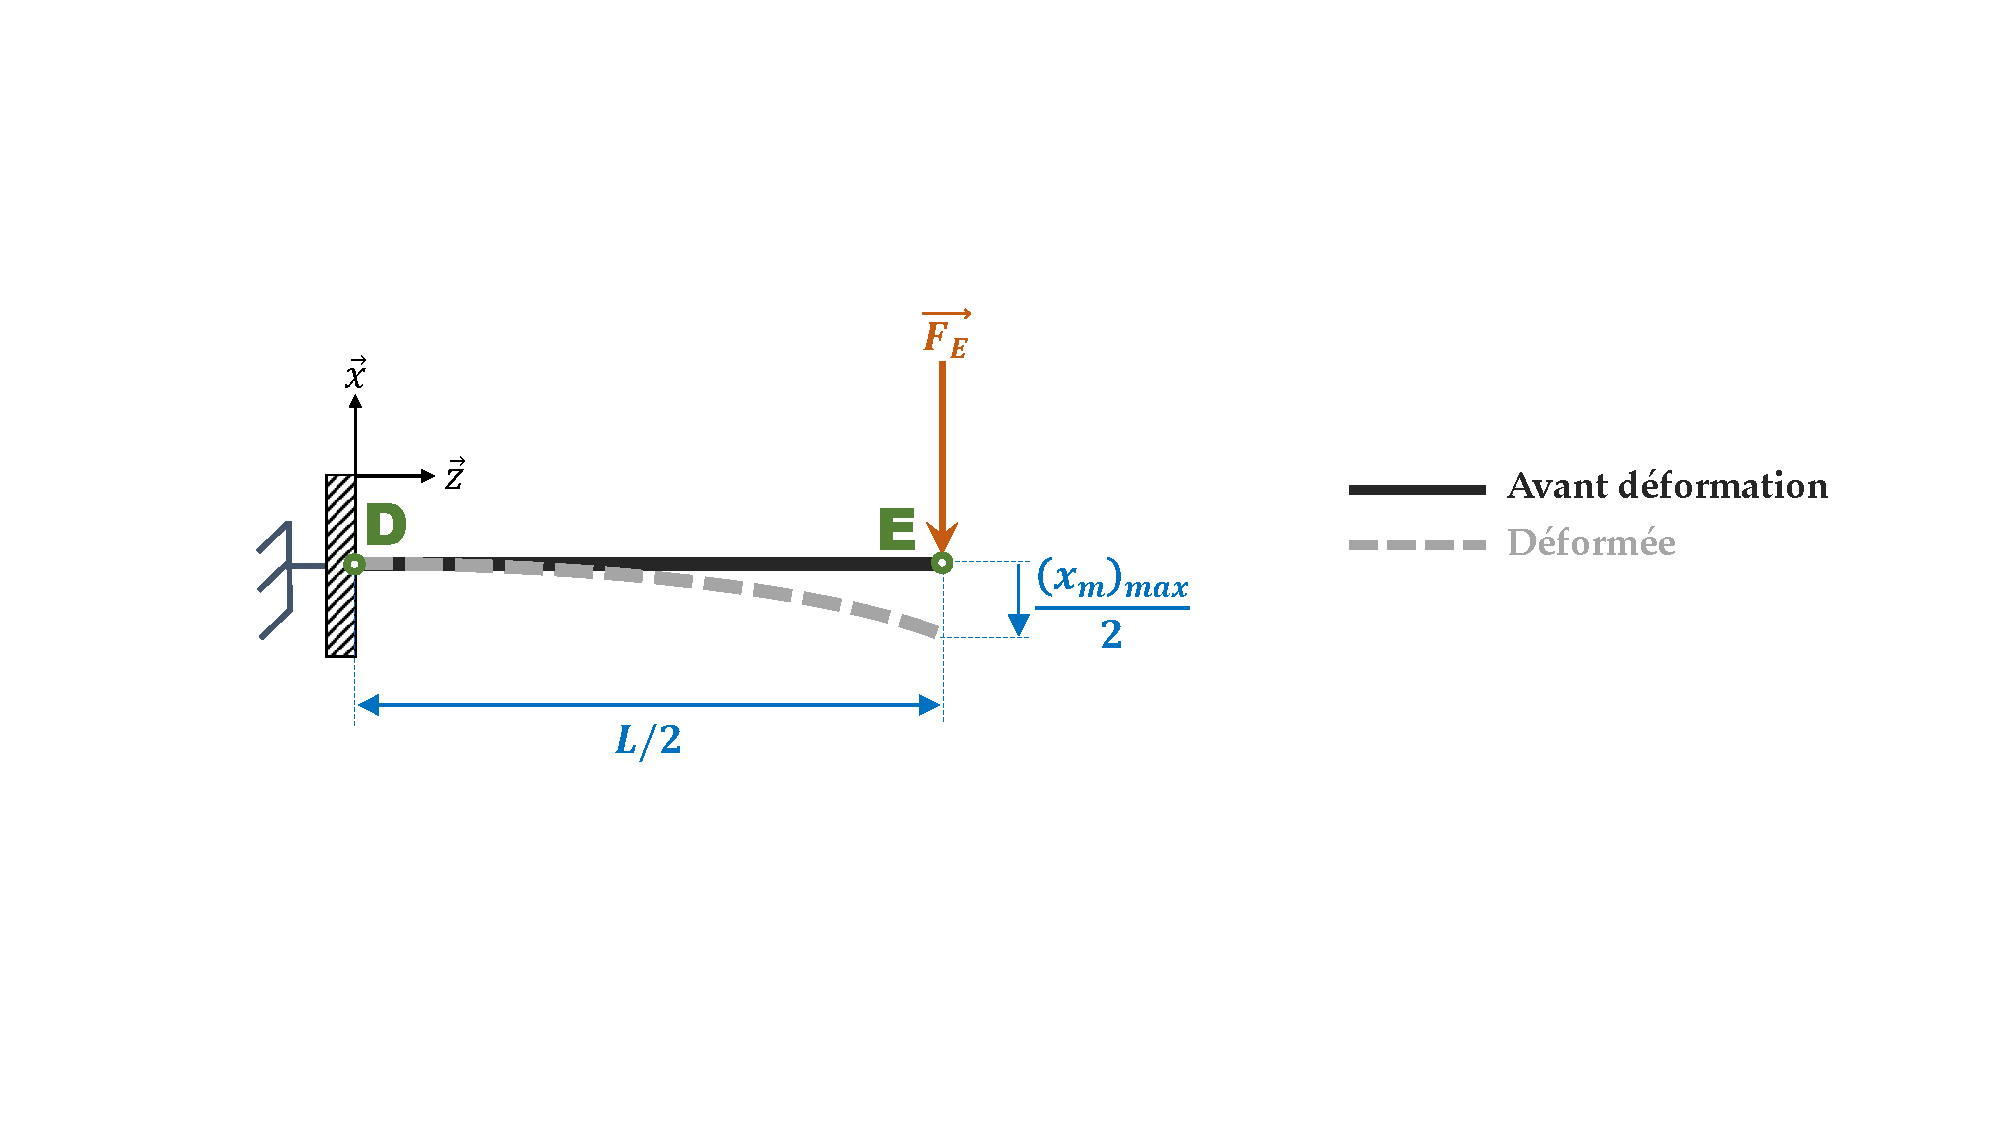
\includegraphics[trim={4cm 5.5cm 2.9cm 5cm},clip, width=\textwidth]{../Chap4/Figure/poutre_flexion_simple.pdf}
	\caption{Schéma poutre encastrée-libre en flexion simple}
	\label{fig:poutre_flexion_simple}
\end{center}
\end{figure}
%%%%%%%%%%%
L'équation de la déformée suivant de la lame suivant z peut alors être exprimée comme suit:
\begin{equation}
		x(z) = \frac{F_E}{6\ E\ I_h}\ z^2 \biggl( \frac{L}{2} - z \biggr)
\label{eq:deformée_encastrée-libre}
\end{equation} 
Où $I_h$ est le moment quadratique d'une lame horizontale. De cette équation on peut alors extraire la flèche maximale qui est à l'extrémité libre en $z=L/2$ :
\begin{equation}
		x_E = \frac{F_E\ (L/2)^3}{3\ E\ I_h}
\label{eq:fleche_encastrée-libre}
\end{equation} 	
De même, on peut exprimer la contrainte normale en flexion $\sigma _f$ grâce à l'équation :
\begin{equation}
	\sigma _f(z) = \frac{-F_E\ (L/2 - z)}{I_h}\ \biggl( \frac{e}{2} \biggr)
\end{equation}

D'autre part on peut exprimer la rigidité en rotation $K_{\varphi 2}$ d'une demi-lame qui est simplement le rapport du moment généré par l'angle de flexion :
\begin{equation}
		K_{\varphi 2} =  \frac{F_E\ (L/2)}{\arctan \biggl( \frac{(x_m)_{max}}{L} \biggr)}
\label{eq:K_phi demi-lame}
\end{equation}
$\varphi$ étant très faible on peut linéariser l'équation  \ref{eq:K_phi demi-lame} pour avoir :
\begin{equation}
		K_{\varphi 2} =  \frac{F_E\ L^2}{2\ (x_m)_{max}}
\label{eq:K_phi demi-lame linéarisée}
\end{equation}
En combinant alors les équations \ref{eq:x_E=x_max/2}, \ref{eq:K_phi_lim} et \ref{eq:K_phi demi-lame linéarisée} on peut exprimer la rigidité en rotation d'une demi-lame en fonction de ses paramètres géométriques et matériau comme suit :
\begin{equation}
		K_{\varphi 2} = \frac{6\ E\ I_h}{L}
		\label{eq:K_phi demi-lame final}
\end{equation}
Un lame complète est donc deux fois plus rigide, et donc :
\begin{equation}
		K_{\varphi} = \frac{12\ E\ I_h}{L}
		\label{eq:K_phi lame entière final}
\end{equation}

    	%*************
		\subsection{Validation du modèle analytique par l'approche numérique} 
		%*************					
On veut valider le modèle analytique établi précédemment par un modèle numérique ANSYS en cherchant à superposer la déformée et la contrainte normale en flexion pour les deux modèles.\\
Le modèle numérique en EF est par conséquent le même que celui qui a été présenté sur la figure \ref{fig:ANSYS_deformation}. On peut alors retrouver sur la figure \ref{fig:comparaison_ANSYS_analytique}
la mise en parallèle des résultats des deux modèles, analytique et numérique.
%%%%%%%%%%%
\begin{figure}[!htbp]
\begin{center}
    \captionsetup{justification=centering}
	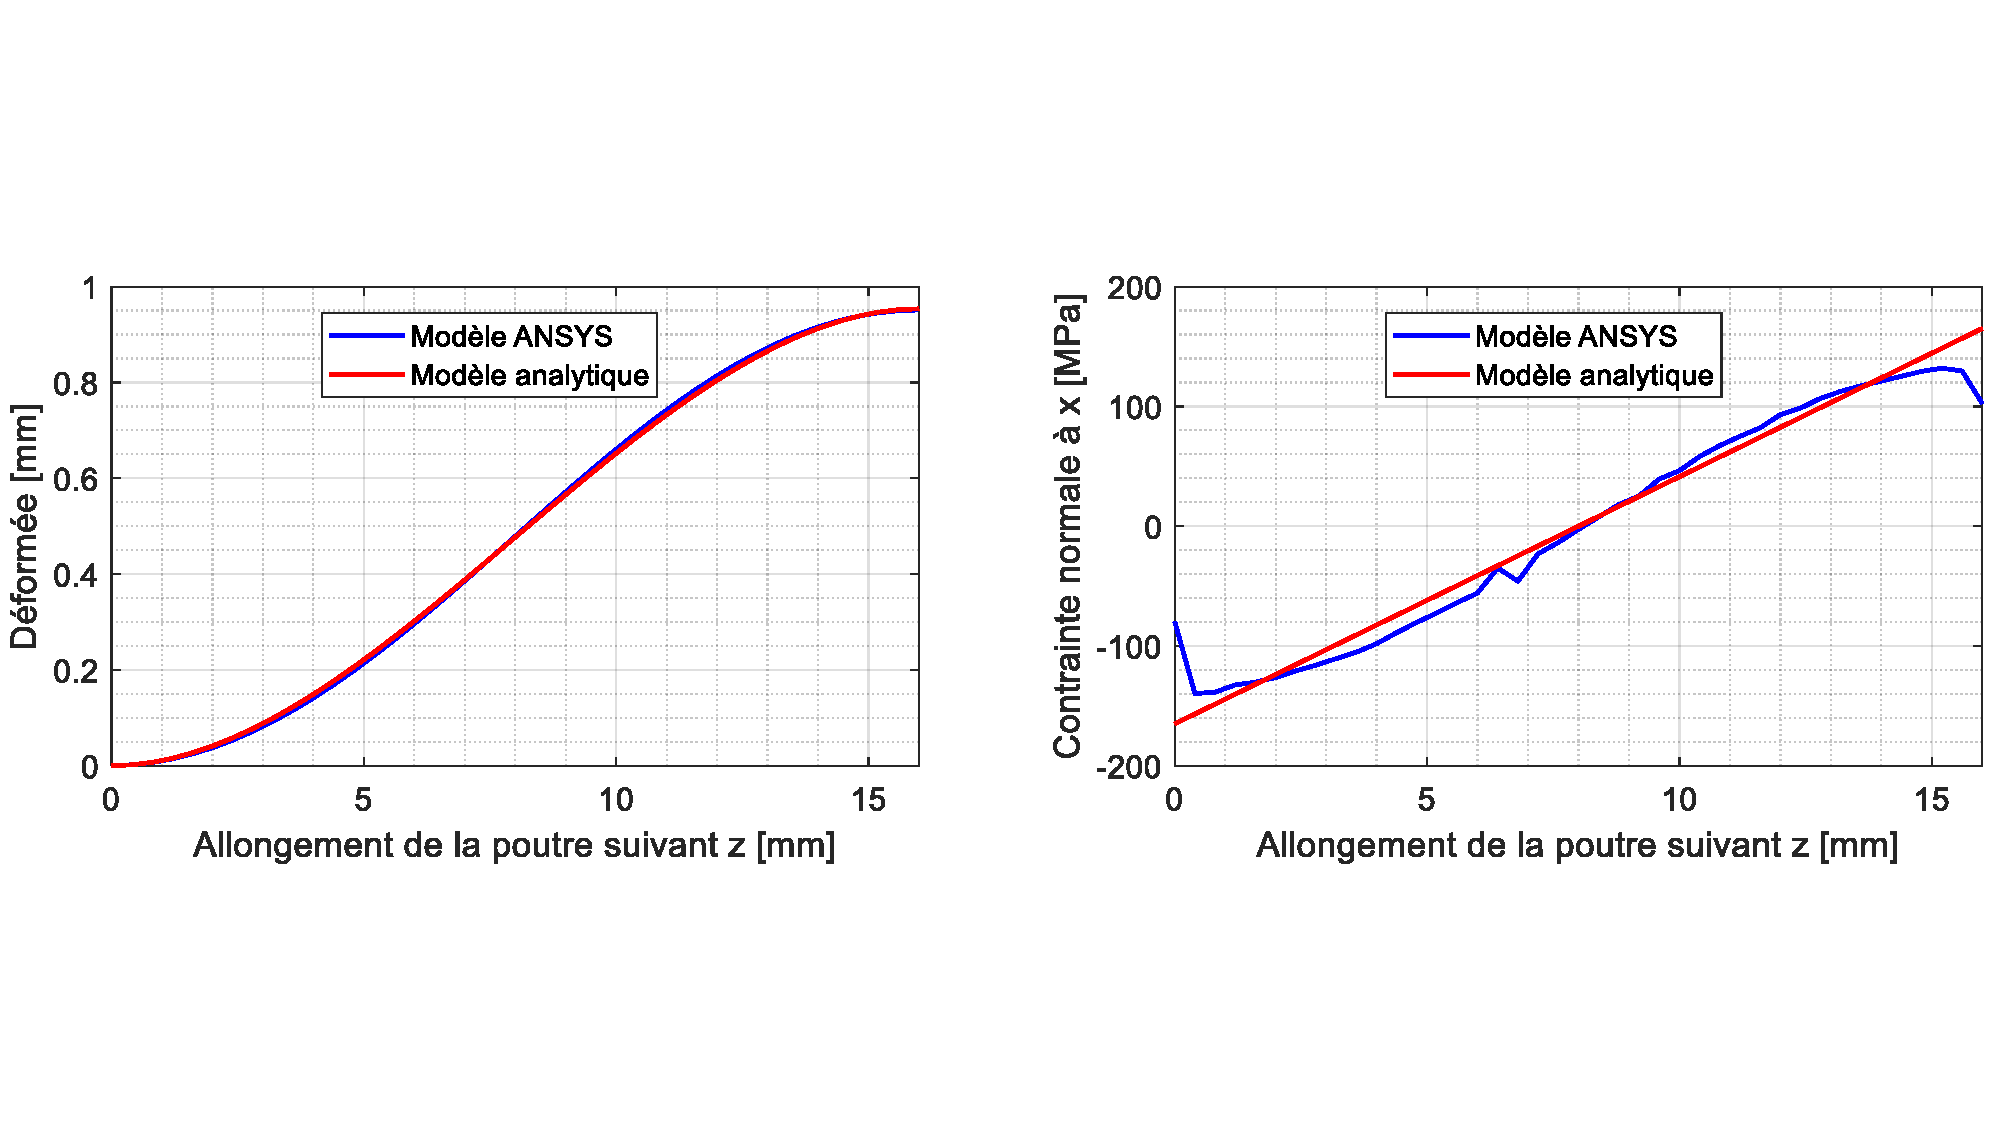
\includegraphics[trim={0cm 4cm 0cm 4.5cm},clip, width=\textwidth]{../Chap4/Figure/comparaison_ANSYS_analytique.pdf}
	\caption{Comparaison de la déformée et de la contrainte normale en flexion entre le modèle analytique et le modèle numérique}
	\label{fig:comparaison_ANSYS_analytique}
\end{center}
\end{figure}
%%%%%%%%%%%
On aperçoit que la déformée est presque identique entre les deux modèles. La tendance et l'ordre de grandeur pour la contrainte normale en flexion dans la fibre supérieure est également similaire entre les deux modèles. On relève notamment que la différence devient plus notable aux points d'ancrages de la lame. Cette différence peut être expliquée par la présence de congés sur le modèle numérique, à l'inverse du modèle analytique.\\
Nous avons dans cette section développé un modèle analytique du comportement mécanique d'un OB suivant l'architecture présentée.

%/!\/!\/!\/!\/!\/!\/!\/!\/!\/!\/!\/!\/!\/!\/!\/!\/!\/!\/!\/!\/!\/!\/!\/!\%
\section{Limite structurelle pour la hauteur de flambement}
\label{sec:3.3_Limite structurelle pour la hauteur de flambement}
%/!\/!\/!\/!\/!\/!\/!\/!\/!\/!\/!\/!\/!\/!\/!\/!\/!\/!\/!\/!\/!\/!\/!\/!\%
 
    %///////////////////////////////////////////// 		
	\subsection{Approche analytique}
	\label{sec:3.3.1_Approche analytique flambement LH}
    %/////////////////////////////////////////////	
Le prototype d'OB présenté dans le chapitre précédent admet une hauteur de flambement limite lorsque celui-ci est seul. En effet, les lames horizontales(LH) du modèle développé assument une rigidité infinie en compression, ce qui serait l'idéal pour transmettre tous les efforts au GPA et maximiser de ce fait le coefficient de couplage du système. L'effort de compression $F_z$ généré sur l'axe $\vec{z}$ de l'OB au passage de $x=0$ doit alors éviter le flambage local des LH. La figure \ref{fig:schema_compression_GPA} illustre le problème en schématisant l'OB en position stable et en position neutre à $x=0$. La compression $\Delta z$ ainsi générée induit $F_z$ qui doit dans le cas idéal être complètement absorbé par le GPA.
%%%%%%%%%%%%%%%%%%%%%%%%%%%%%%%%%%%%	
\begin{figure}[!htb]
\begin{center}
    \captionsetup{justification=centering}
	\includegraphics[trim={0cm 0cm 0cm 5cm},clip, 					                 width=0.8\textwidth]{../Chap5/Figure/schéma_compression_GPA.pdf}
	\caption{Détail d'une lame horizontale du prototype d'OB conçu}
	\label{fig:schema_compression_GPA}
\end{center}	
\end{figure}    
%%%%%%%%%%%%%%%%%%%%%%%%%%%%%%%%%%%%
Cet effort peut être évalué pour $x_0$ fixe par l'équation \ref{eq:F_z}.
\begin{equation}
	F_z\ =\ K\ \Delta z\ =\  K\ 2(\sqrt{({x_0}^2+L^2)} - L)
	\label{eq:F_z}
\end{equation}  
D'autre part, on peut évaluer la force de flambage critique d'Euler $F_{ce}$ \cite{Bourahla2011}, au delà de laquelle les LH flamberaient. Celle-ci s'exprime par l'équation \ref{eq:Fce_Euler}.
\begin{equation}
	F_{ce} = \dfrac{{\pi}^2\ E\ I_{min}}{\mu_c\ l^2}
	\label{eq:Fce_Euler}
\end{equation}
Où $E$ est le module d'élasticité du matériau, $l$ est la longueur de la poutre et $I_{min}$ est l'inertie dans la direction la plus faible, exprimée par l'équation \ref{eq:I_min} pour nos lames de section $l$ x $e$ qu'on a répertorié dans le tableau \ref{tab:parametres_lames}.
\begin{equation}
	I_{min} = \dfrac{e\ l^3}{12} = \dfrac{1.2{e-3}\ \cdot\ {(75e^{-6})}^3}{12} = 4.22e^{-5}\ \text{mm}^4
	\label{eq:I_min}
\end{equation}
Enfin, $\mu_c$ est un coefficient qui dépend des conditions initiales. Pour ce qui est de notre prototype, sur la figure \ref{fig:detail_poutre_horizontale} on trouve le détail d'une des 4 LH identiques constituant l'OB. On doit alors déterminer la longueur de flambage et les conditions initiales qui s'appliquent à notre cas.
%%%%%%%%%%%%%%%%%%%%%%%%%%%%%%%%%%%%	
\begin{figure}[!htb]
\begin{center}
    \captionsetup{justification=centering}
	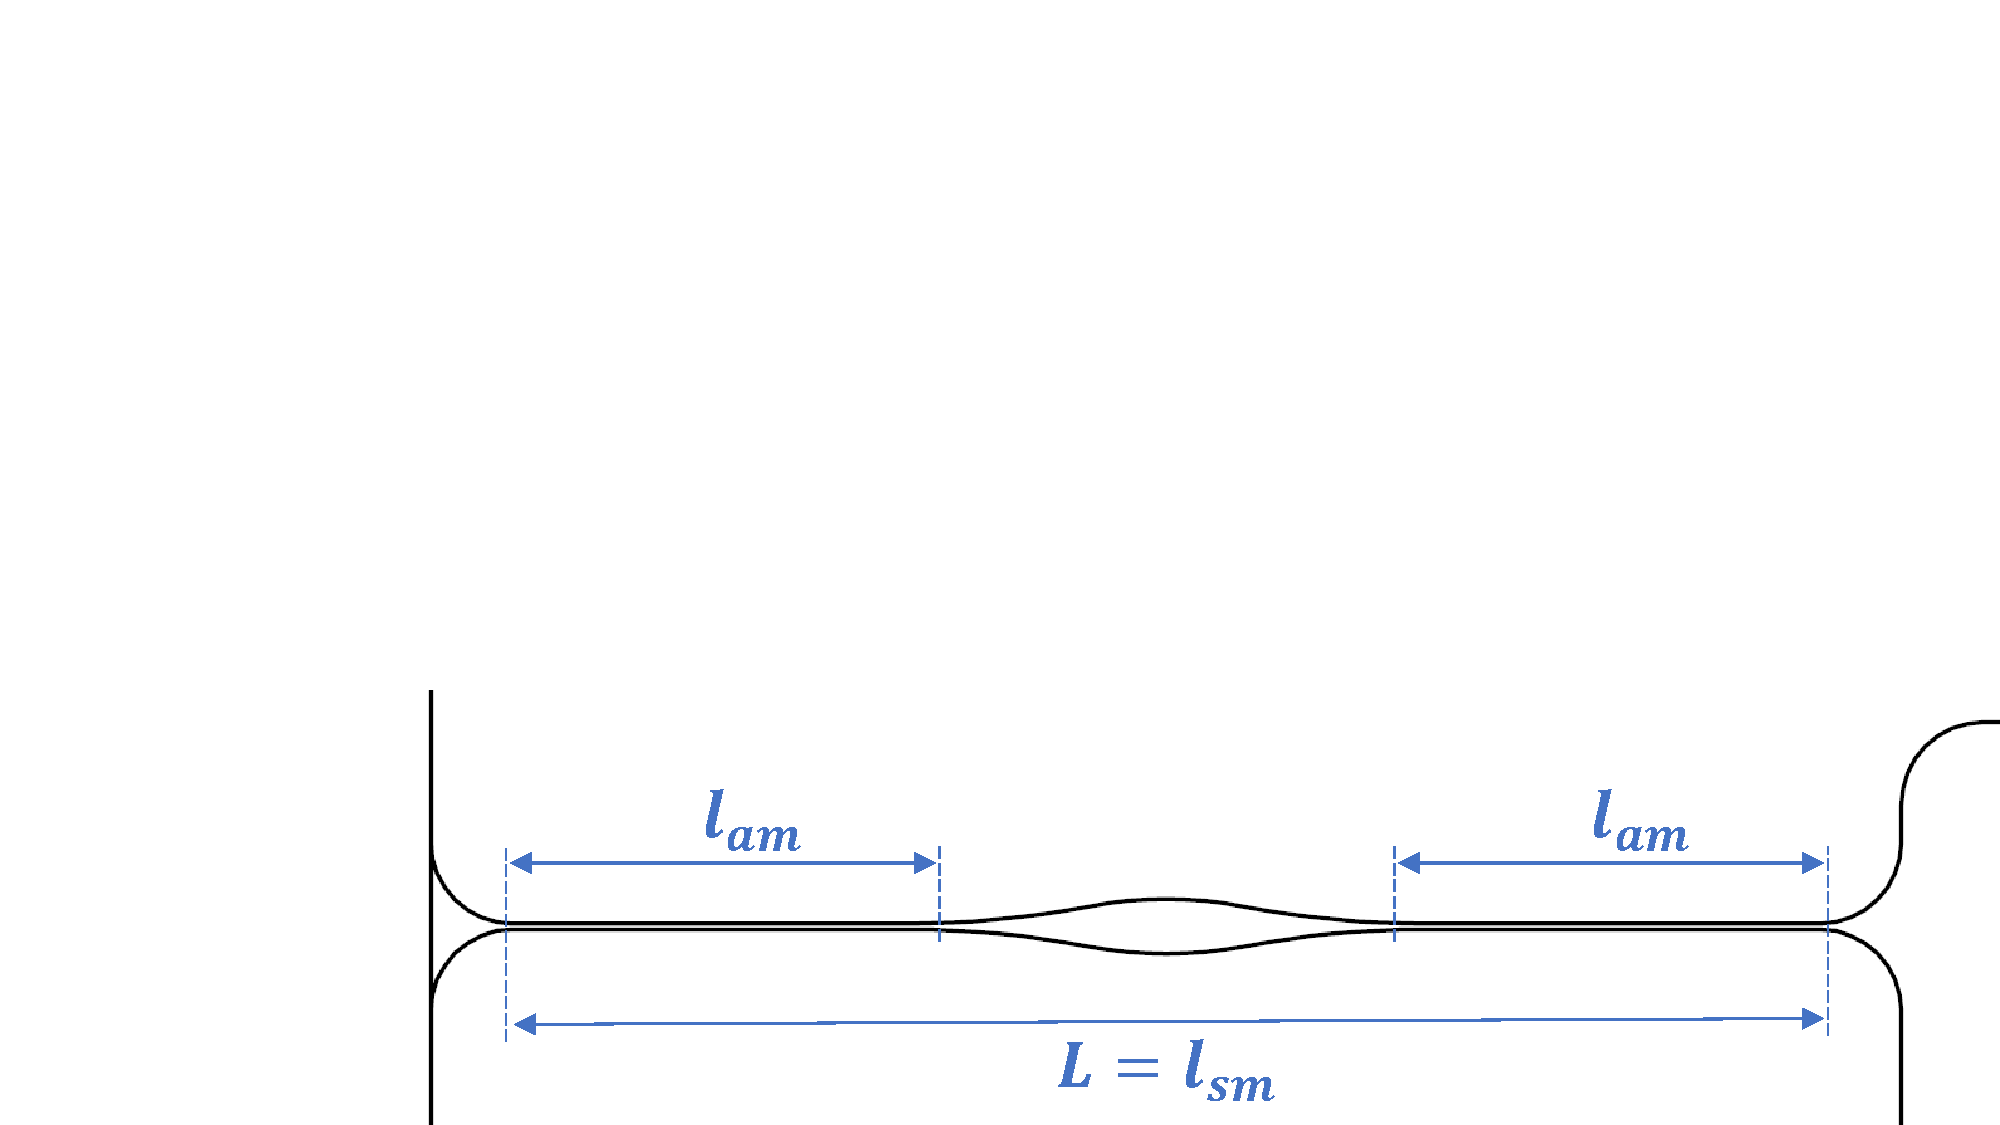
\includegraphics[trim={7cm 0cm 0cm 12cm},clip, 					                 width=0.6\textwidth]{../Chap5/Figure/detail_poutre_horizontale.pdf}
	\caption{Détail d'une poutre horizontale du prototype d'OB conçu}
	\label{fig:detail_poutre_horizontale}
\end{center}	
\end{figure}    
%%%%%%%%%%%%%%%%%%%%%%%%%%%%%%%%%%%%  
On suppose que l'épaississement local sur les LH induira obligatoirement le flambement sur les portions les plus fines desquelles il est entouré. Une telle conception permettrait alors de réduire le risque d'apparition du flambage sur toute la longueur de la poutre. En effet, cela réduirait la longueur de flambage de $l_{sm}=L=16$mm à $l_{am}=4.82$mm. D'autre part, en nous référant aux ouvrages sur la résistance des matériaux \cite{Bourahla2011}, on présente certaines valeurs de $\mu_c$ en fonction de différentes conditions initiales sur la figure \ref{fig:detail_poutre_horizontale}.
%%%%%%%%%%%%%%%%%%%%%%%%%%%%%%%%%%%%	
\begin{figure}[!htb]
\begin{center}
    \captionsetup{justification=centering}
	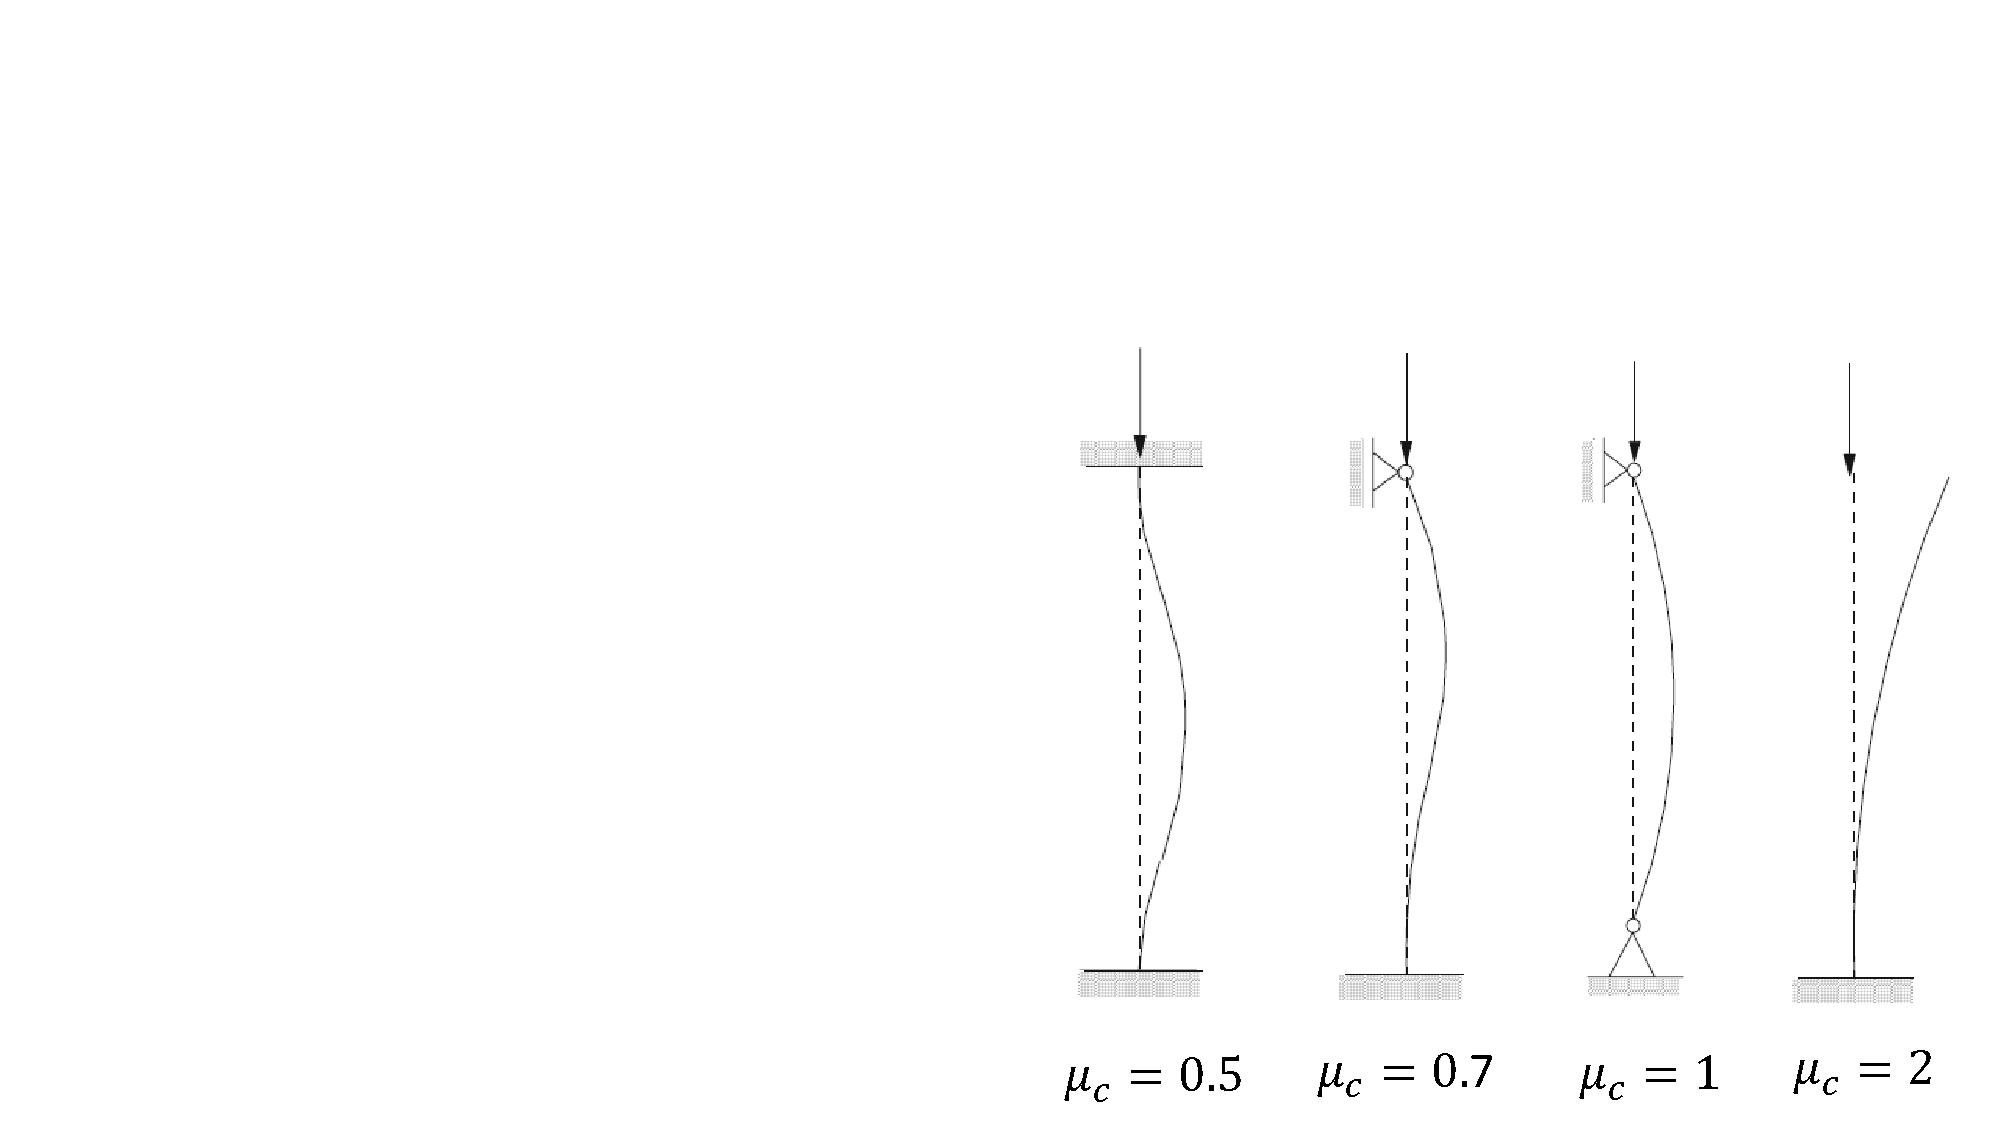
\includegraphics[trim={15cm 0cm 0cm 6cm},clip, 					                 width=0.6\textwidth]{../Chap5/Figure/CI_flambement.pdf}
	\caption{Valeur de $\mu_c$ pour différentes conditions initiales de flambage \cite{Bourahla2011}}
	\label{fig:CI_flambement}
\end{center}	
\end{figure}    
%%%%%%%%%%%%%%%%%%%%%%%%%%%%%%%%%%%% 
Les conditions initiales de flambement vont varier en fonction de la présence ou non de masselotte centrale sur les LH. Dans le cas avec masselotte, chacune des deux portions de lame de longueur $l_{am}$ se rapprochent du cas encastrée-libre où $\mu_c=2$. Pour le cas sans masselotte on suppose qu'on se trouve plutôt dans la configuration encastré-encastré où $\mu_c=0.5$. On peut alors évaluer $F_{ce}$ avec pour chacun des deux cas en connaissant les dimensions exactes du prototype.
En addition, l'effort de compression sur le GPA est repris par 4 lames identiques sur l'OB, ce qui répartit équitablement $F_z$ sur chacune d'elles. On doit donc s'assurer que le coefficient de sécurité de flambage ${s_f}$ défini à l'équation \ref{eq:Fz/4Fce} pour une seule lame soit inférieur à 1.
\begin{equation}
		s_f\ =\ \dfrac{F_z}{4\ F_{ce}}
		\label{eq:Fz/4Fce}
\end{equation}
On peut alors déterminer la hauteur limite structurelle de flambement $x_{0m}$ de l'OBs avec en combinant les équations \ref{eq:F_z}, \ref{eq:Fce_Euler} et \ref{eq:Fz/4Fce} dans l'équation \ref{eq:x_0m}.
\begin{equation}
	x_{0m} =\sqrt{ \biggl(\frac{2\ \pi^2\ E\ I_{min}}{K\ \mu_c\ l_l^2}\ +\ L\biggr)^2\ -\ L^2}
	\label{eq:x_0m}
\end{equation}
Avec les dimensions du prototype conçu et les propriétés mécanique tirées de la documentation technique du GPA(APA50XS), on estime $x_{0m}=0.63$mm. Si on avait choisi de concevoir l'OB sans les masselottes, la hauteur de flambement maximale serait réduite à $0.37$mm pour une même longueur de lame $L$.\\
	En imposant alors un flambement supérieur à $x_{0m}$ , on risque de détériorer le coefficient de couplage du système, et par extension, le rendement global de conversion d'énergie. Cet aspect devra être recalculé avec la validation expérimentale de la raideur apparente du prototype.		
	
    	%*************
		\subsection{Corrélation analytique - numérique} 
		%*************		
%%%%%%%%%%%%%%%%%%%%%%%%%%%%%%%%%%%%	
\begin{table}[!htbp]
	\centering
		\begin{tabular}[t]{|c|c|m{1cm}|m{1cm}|}
\hline
\multicolumn{2}{|c|}{\multirow{2}{*}{\textbf{Paramètres}}} & \multicolumn{2}{c|}{\textbf{Architecture OB}}\\
\cline{3-4} 
\multicolumn{2}{|c|}{} &
 \multicolumn{1}{c|}{\textbf{SM}} &
  \multicolumn{1}{c|}{\textbf{AM}} \\
\hline \hline
\multirow{3}{*}{Hypothèse analytique} &  $\mu_c$ [~~]	& 0.5  & 2  \\
\cline{2-4} 
									  &  $F_{ce}$ [N]  & 0.69 & 1.9 \\\cline{2-4} 
									  &  $x_{0m}$ [mm]  & 0.41 & 1.6 \\

\hline
\multirow{3}{*}{Correction numérique en EF} & $\mu_c$ [~~]  & 0.64 & 2.36 \\
\cline{2-4} 
									 		& $F_{ce}$ [N]  & 0.54 & 1.6 \\	\cline{2-4} 
										    & $x_{0m}$ [mm] & 0.37 & 0.63 \\
									   
\hline
		\end{tabular}
        \caption{Comparaison des facteurs de CI pour les architectures SM et AM avant et après corrélation analytique-numérique}
        \label{tab:corection_CI_flambement}
\end{table}        
%%%%%%%%%%%%%%%%%%%%%%%%%%%%%%%%%%%%	
En nous appuyant sur les résultats de l'étude EF, on peut venir corriger le modèle analytique en recalant les hypothèses des conditions initiales. En effet, cela revient à modifier le coefficient $\mu_c$ dans l'équation \ref{eq:x_0m} afin de trouver l'égalité de la charge critique d'Euler entre les deux modèles, définis respectivement aux équations \ref{eq:Fce_Euler} et  \ref{eq:Euler_EF}. Le coefficient de condition initiale $\mu_c$ peut maintenant être corrigé en remplaçant $F_{ce}$ par les résultats du modèle EF. On liste alors dans le tableau \ref{tab:corection_CI_flambement} les facteurs de CI des hypothèses de départ, ainsi que ceux calculés d'après les résultats des simulations EF. \\
On en déduit, en comparant les hypothèses et les corrections numériques, que le modèle analytique est proche des prédictions du modèle EF. Cependant, pour les deux cas de figures SM et AM, le modèle analytique est sous-dimensionné. Le modèle numérique est donc à privilégier pour une dimensionnement en flambage car les hypothèses au CI sont difficiles à prédire analytiquement au vu de l'architecture complexe de poutres en déformation.
		